
\chapter{Introduction}\label{r:introduction}

The remarkable success of deep neural networks in computer vision has been accompanied by an equally pressing need to understand their decision-making processes. As these models are deployed in critical applications ranging from medical diagnosis to autonomous driving, the ability to explain and interpret their behavior becomes paramount for building trust, ensuring fairness, and identifying potential failure modes.

Current explainable AI (XAI) methods have made significant strides in providing insights into model behavior through various approaches including saliency maps \citep{simonyan2014deepinsideconvolutionalnetworks}, concept activation vectors \citep{kim2018interpretabilityfeatureattributionquantitative}, and gradient-based attribution methods \citep{sundararajan2017axiomaticattributiondeepnetworks}. However, these approaches share a fundamental limitation: they primarily operate within the confines of known training data or slight perturbations thereof, leaving vast regions of the input manifold unexplored.

More recent advancements that expand the scope of interpretability try to address those limitations. Approaches such as Rate-Distortion Explanation (RDE) frameworks systematically perturb input signals across diverse data modalities to identify truly relevant features, thereby moving beyond local sensitivity \citep{Kolek2022}. These frameworks also explicitly aim for in-distribution interpretability by leveraging generative models like in-painting GANs, thereby guarding against explanations corrupted by evaluations in undeveloped or unrealistic regions of the model's function. Similarly, new techniques for interpreting deep generative models (GANs) enable the identification of human-understandable concepts within latent spaces, allowing for interactive image generation and editing. This actively explores the input manifold by creating new data, offering insights into how realistic images are composed from deep representations. \citep{zhou2022interpretinggenerativeadversarialnetworks, Karimi2022}

Furthermore, XAI is seeing a shift towards building transparency into models from the outset, often referred to as "interpretable-by-design" methods \citep{Karimi2022, Holzinger2022a}. Research into interpretable reinforcement learning via programmatic policies aims to train policies in the form of human-readable programs (e.g., decision trees, state machines), which are inherently more interpretable, verifiable, and robust than traditional deep neural network policies \citep{inbook, Inala2020Synthesizing, verma2019programmaticallyinterpretablereinforcementlearning}. Likewise, Explainable Neural-Symbolic Learning (X-NeSyL) represents another design-based approach, fusing deep learning representations with expert knowledge graphs to encourage neural networks to learn structures akin to human expert reasoning, ensuring interpretability is embedded throughout the training process \citep{D_az_Rodr_guez_2022, karimi2020algorithmicrecoursecounterfactualexplanations}.

These advancements align with what is sometimes referred to as "RED XAI" – a model-centric culture focused on questioning models, extracting knowledge, spotting, and fixing bugs, and ultimately improving the reliability and safety of AI systems \citep{10.5555/3692070.3692231}. This perspective is critical for using explanations not just to justify decisions, but to drive model development and verification \citep{Tsai2022}. This includes attributing importance to feature interactions and groups, which can then be used to directly improve model generalization or to distill complex models into simpler forms, often validated through "reality checks" \citep{Singh2022}
\section{Motivation and Problem Statement}

Consider a trained image classifier that correctly identifies both a standard photograph of a dog and a highly stylized artistic rendering of the same animal. Traditional XAI methods would analyze these two specific instances, potentially identifying common features like shape or texture patterns. However, they would miss the broader question: what other visual representations would this model also classify as a dog with the same confidence?

The phrase "a dog with the same confidence" refers to something far more profound and potentially disturbing than might initially appear. This concept extends beyond different breeds of dogs, dogs photographed from different angles, or even dogs rendered in different artistic styles. The phenomenon encompasses the complete universe of visual patterns—no matter how bizarre, abstract, or seemingly unrelated to dog anatomy—that trigger identical neural responses in the classifier's decision-making apparatus. This could include a Jackson Pollock painting with just the right splatter of paint, a close-up photograph of tree bark with particular texture patterns, a geometric arrangement of colored pixels that bears no resemblance whatsoever to any living creature, or even a photograph of a kitchen appliance that happens to contain the precise combination of edges, curves, and color distributions that the model has learned to associate with "dog-ness." The classifier assigns these wildly disparate inputs exactly the same probability score—perhaps 0.8347 for "dog"—despite their complete lack of semantic relationship to actual dogs.

This question is not merely academic but reveals a fundamental blindness in our understanding of machine learning models. Traditional explainable AI methods focus on the narrow slice of reality represented in training datasets, leaving vast territories of the input manifold completely unexplored and potentially harboring unexpected model behaviors. The robustness implications are staggering: if a model can be fooled into seeing a dog in a random arrangement of geometric shapes with the same confidence as it sees a dog in an actual photograph of a Golden Retriever, what does this say about its reliability in real-world deployment? The bias detection possibilities are equally concerning—systematic patterns within these datasets might reveal that the model has learned to associate certain irrelevant features (perhaps related to image compression artifacts, camera settings, or demographic markers in the background) with specific classes, perpetuating hidden biases that would never be discovered through traditional dataset analysis. For fairness evaluation, understanding these equivalence classes becomes critical: if the model makes identical predictions for inputs that vary along protected attributes while maintaining other spurious correlations, we need to map these relationships to ensure equitable treatment. Finally, the structure of these datasets provides unprecedented insight into how models generalize beyond their training distribution—revealing whether generalization relies on semantically meaningful features or on arbitrary statistical regularities that happen to correlate with class labels in the training data.

\section{Proposed Approach: Generative Explainable AI}

This thesis introduces a paradigm shift from traditional interpolative XAI methods to a generative approach. Instead of analyzing existing data points, this work proposes synthesizing new, meaningful examples that preserve model predictions, thereby exploring the \textit{Invariant Set} -- the complete collection of inputs that yield identical outputs under a given objective function.

The proposed method combines score-based generative models with classifier guidance to sample high-quality, diverse images from these invariant sets. By leveraging the powerful generative capabilities of diffusion models, one can explore regions of the input space that may never have been encountered during training, providing a more comprehensive understanding of model behavior.

Figure~\ref{fig:1_teaser} illustrates the conceptual distinction between proposed approach and current XAI methods. While traditional methods focus on explaining decisions within known data boundaries, generative XAI does not have this limitation and can explore the broader space of possible inputs that lead to the same predictions.

\begin{figure}[h]
\centering
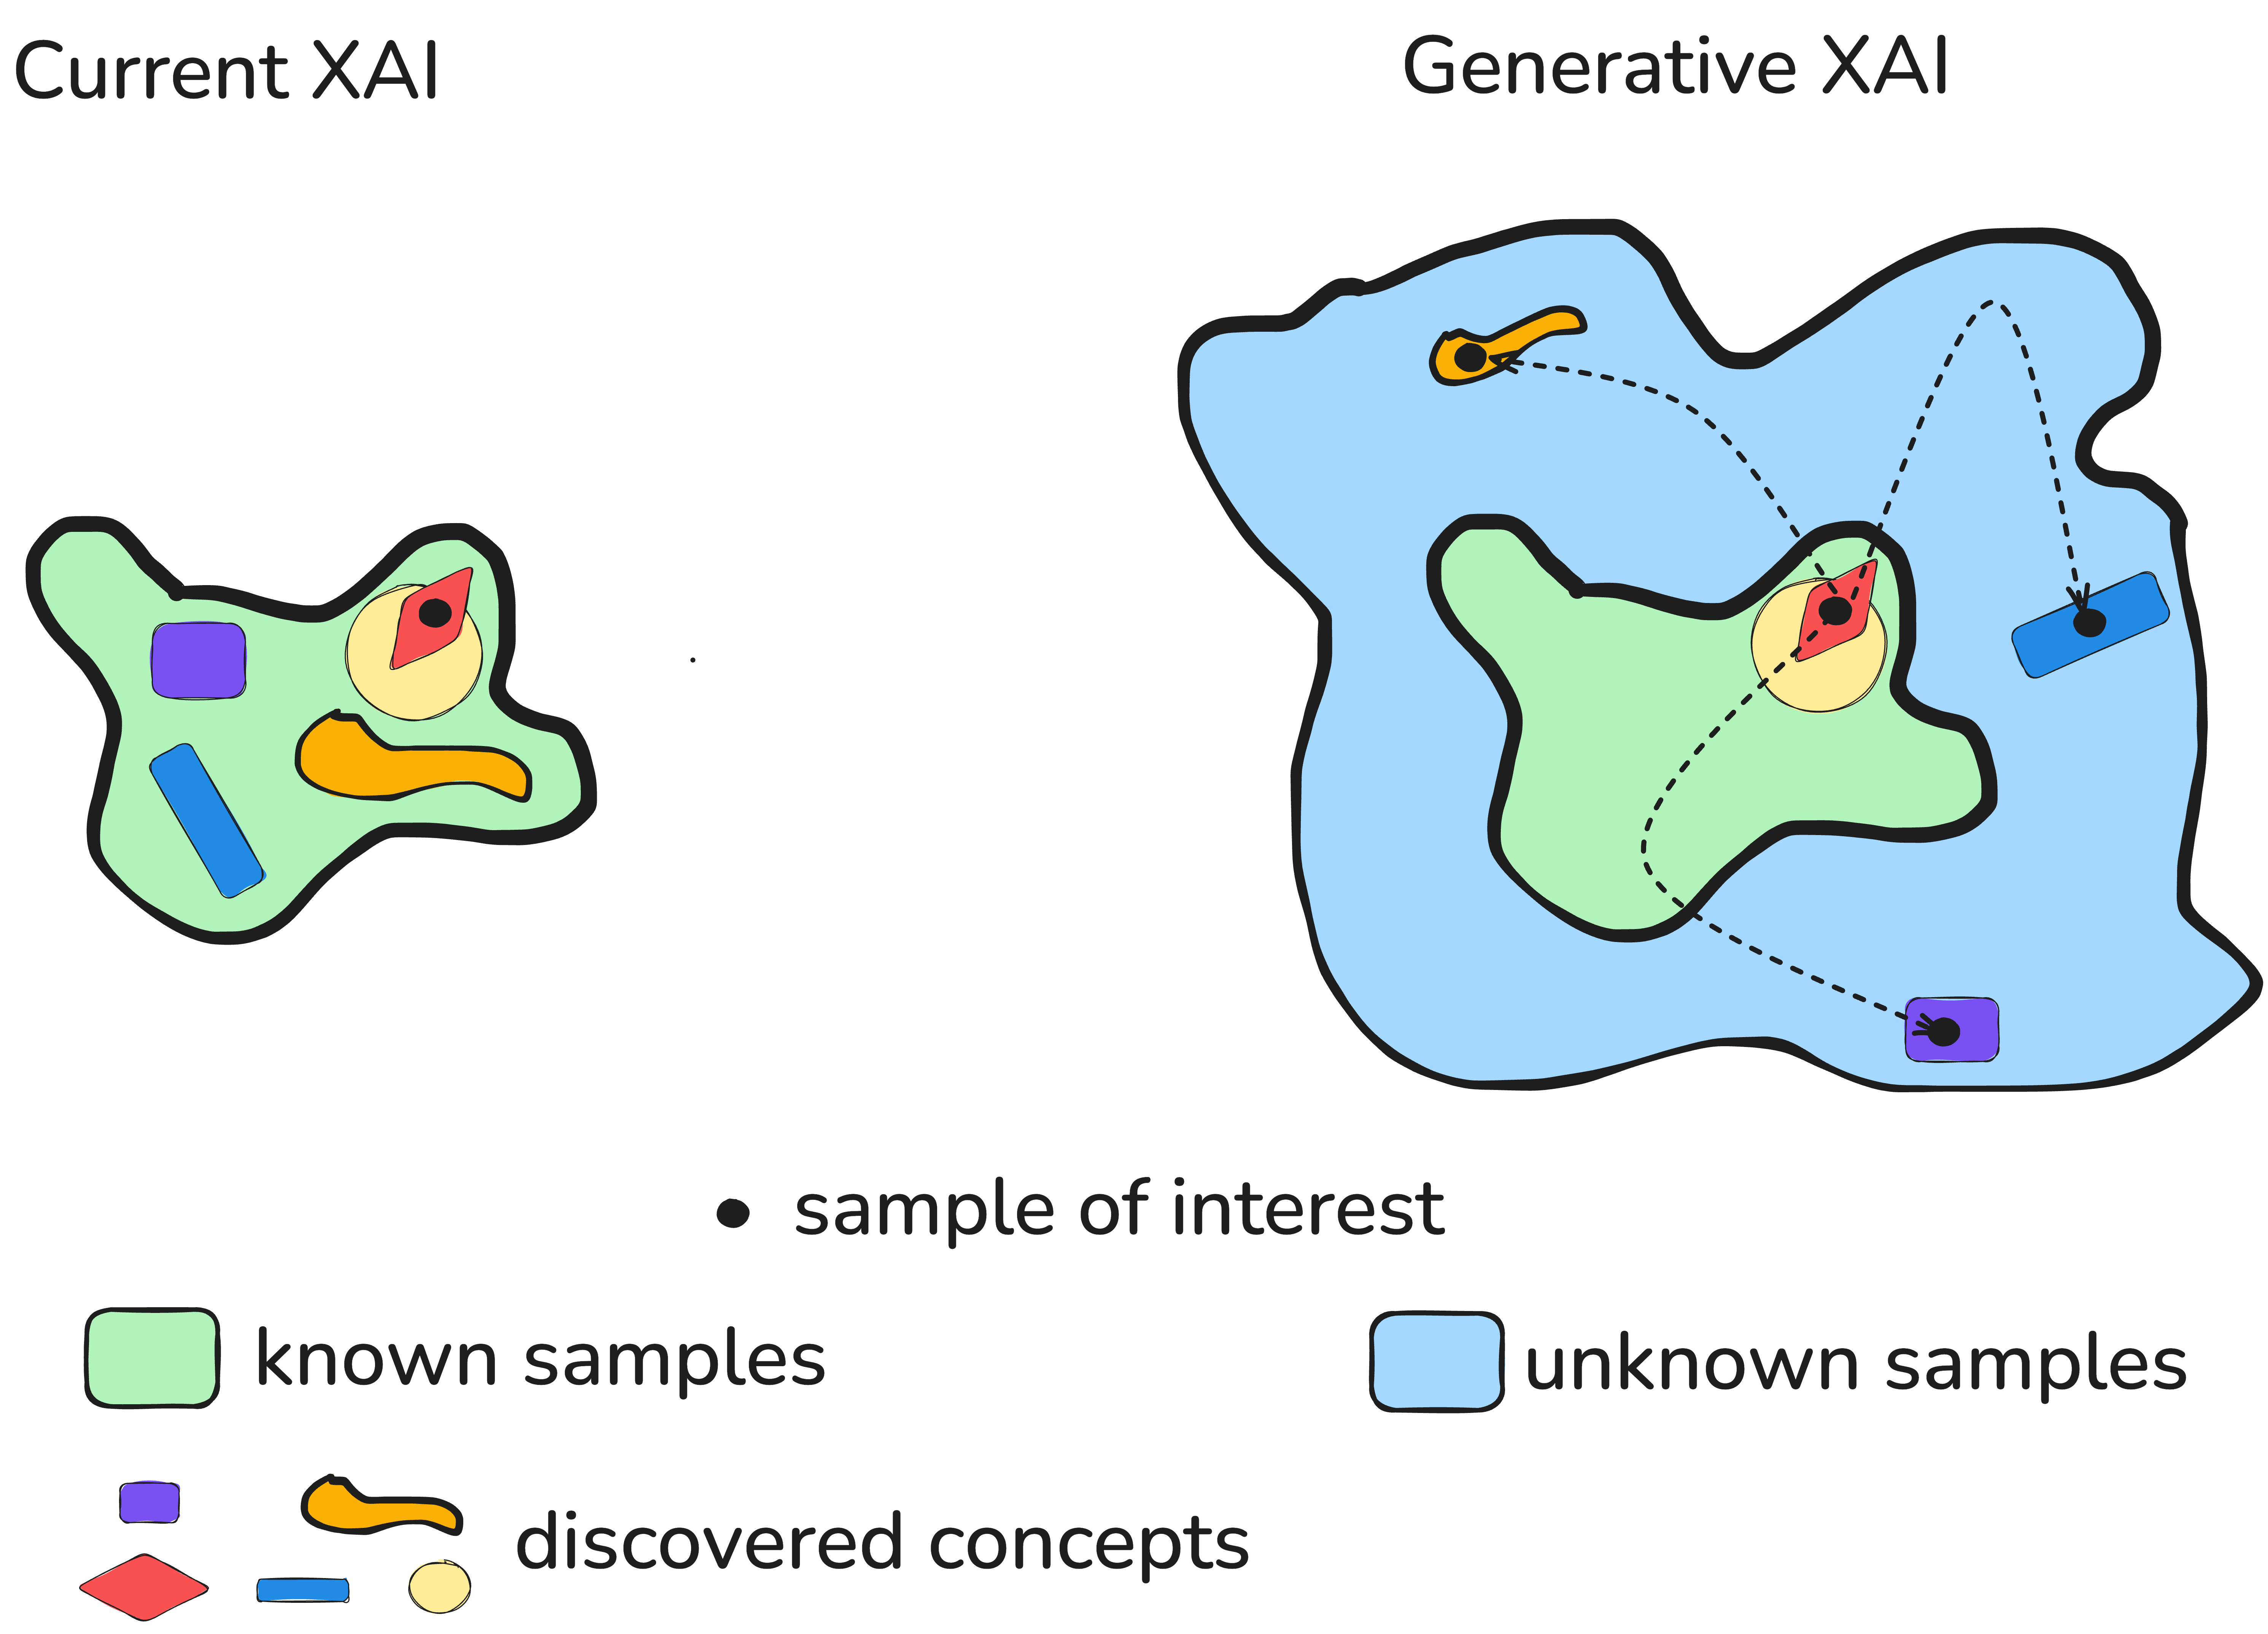
\includegraphics[width=0.8\linewidth]{figures/main/teaser1.png}
\caption{Conceptual comparison between traditional XAI methods and Generative XAI. Traditional methods analyze known data samples (left), while proposed approach synthesizes diverse examples from the invariant set that yield identical predictions (right).}
\label{fig:1_teaser}
\end{figure}

\section{Contributions}

This thesis makes three key contributions to the field of explainable AI, as outlined in the abstract and detailed in Chapter~\ref{r:method}:

The first contribution represents a \textbf{paradigm shift from traditional explainable AI methods} that analyze human-interpretable features in known data samples to generative XAI methods that synthesize new samples. This fundamental change in perspective allows for exploration of vast regions of the input manifold that remain unexplored by current approaches, providing a more comprehensive understanding of model behavior beyond the confines of training datasets.

The second contribution introduces a \textbf{novel theoretical backbone for generative XAI methods}. This framework provides formal mathematical definitions of invariant sets and establishes their properties as equivalence relations, offering a rigorous foundation for understanding and generating diverse examples that yield identical model predictions.

The third contribution presents an \textbf{efficient algorithmic implementation of this framework}. This method combines score-based diffusion models with guided sampling to generate high-quality, diverse examples from invariant sets, enabling practical application of the theoretical framework to real-world neural network analysis and interpretation.

These contributions are comprehensively detailed and evaluated in Chapter~\ref{r:method}, where both the theoretical foundations and empirical validation of proposed approach are presented.

\section{Thesis Organization}

The remainder of this thesis is structured to provide a comprehensive exploration of proposed generative explainable AI approach. Chapter~\ref{r:related_work} reviews the relevant literature across explainable AI methods, generative modeling, and diffusion models, establishing the theoretical foundation for this work. Chapter~\ref{r:method} presents core theoretical framework and details the \method{} algorithm, providing the mathematical foundation for invariant set generation and the practical implementation of proposed approach.

Chapter~\ref{r:experiments} presents a comprehensive experimental evaluation demonstrating the effectiveness of proposed method across multiple neural network analysis paradigms, from individual neuron activation to complete classifier output preservation. Chapter~\ref{r:applications} explores practical applications of this framework in real-world scenarios, while Chapter~\ref{r:discussion} discusses the broader implications of this work, current limitations, and directions for future research. Chapter~\ref{r:conclusion} synthesizes contributions and their significance for the field of explainable AI.
